\section{问题四：收缩域上的移动边界模型}

\subsection{实测半径与物质坐标变换}

本问的求解区域不再固定。附件 2 给出 $145$ 个时刻的药材半径，覆盖 $0$ 至 $259200$~s，半径由 $2.000$~cm 单调减到序列末端的 $1.198$~cm，自 $126000$~s 起即稳定在 $1.200$~cm 附近，序列末端的收缩比为 $0.599$，截面积只剩初始的 $0.3588$；后文用到的停时处收缩比按该时刻的半径另行取值。半径序列的形态见图~\ref{fig:radius-shrink}。

\begin{figure}[htbp]
  \centering
  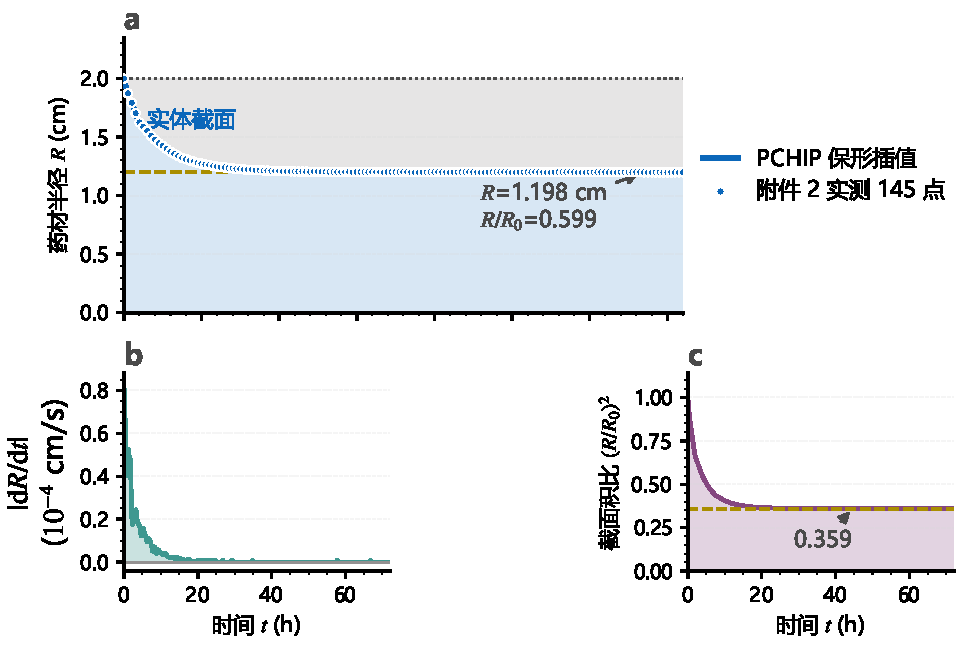
\includegraphics[width=0.9\textwidth,height=0.8\textheight,keepaspectratio]{../figures/fig_radius_shrink.pdf}
  \caption{附件 2 实测的药材半径收缩过程。a：散点为 145 点实测值，曲线为
  PCHIP 保形插值（保形以避免插值曲线出现非物理的半径回弹），深色填充为药材
  实体截面，浅色为已收缩掉的区域；b：收缩速率 $|\mathrm{d}R/\mathrm{d}t|$；
  c：截面积比 $(R/R_0)^2$。终值半径与收缩比直接进入问题 4 的物质坐标变换。}
  \label{fig:radius-shrink}
\end{figure}

收缩集中在前二十小时，此后速率趋于零，这与含水率的前快后慢是一致的：失水停止，收缩自然也停止。热风干燥的实测研究也报告了同一现象，即收缩量与失水量在整个过程中同步演化，且两者共同改变有效扩散系数\upcite{ning2025shrinkage}。插值方式的选择在此处有实际后果。三次样条会在拐点附近产生过冲，使插值曲线出现半径回升这种非物理的结果；分段三次 Hermite 保形插值则保持原始数据的单调性，导数由插值函数解析求出而非对原始数据作差分，避免出现半小时周期的阶梯脉冲。

区域随时间变形，固定域上的离散格式不能直接套用。本文引入以当前半径归一的物质坐标

\begin{equation}
s=\frac{r}{R(t)}\in[0,1],
\label{eq:mapping}
\end{equation}

在径向仿射收缩下，同一个 $s$ 始终标记同一份干物质，因此 $s$ 是物质标签而非固定于实验室的空间坐标。链式法则给出

\begin{equation}
\left.\frac{\partial C}{\partial t}\right|_{r}
=\left.\frac{\partial C}{\partial t}\right|_{s}
-\frac{s\dot R}{R}\frac{\partial C}{\partial s},
\qquad
\frac{\partial}{\partial r}=\frac{1}{R(t)}\frac{\partial}{\partial s} .
\label{eq:chain}
\end{equation}

把式~\eqref{eq:chain} 代回式~\eqref{eq:mass}，表观对流项与坐标变换产生的项精确相消，剩下纯扩散形式

\begin{equation}
\left.\frac{\partial C}{\partial t}\right|_{s}
=\frac{1}{R^2(t)}\cdot\frac{1}{s}\frac{\partial}{\partial s}
\!\left(s\,D(C,T)\frac{\partial C}{\partial s}\right),
\qquad 0<s<1,
\label{eq:q4c}
\end{equation}

\begin{equation}
\left.\frac{\partial C}{\partial s}\right|_{s=0}=0,
\qquad
\left.-\frac{D(C,T)}{R(t)}\frac{\partial C}{\partial s}\right|_{s=1}
=h_m\big[C(1,t)-C_a(t)\big].
\label{eq:q4bc}
\end{equation}

温度方程同构，只需把 $D$ 换成 $\lambda$、右端整体除以 $\rho c_p$、边界系数换成 $h$ 与 $T_a$。方程中不再出现半径变化率，但收缩并未被忽略：$R(t)$ 出现在式~\eqref{eq:q4c} 的 $1/R^2(t)$、式~\eqref{eq:q4bc} 的 $1/R(t)$ 以及控制体的物理体积 $R^2(t)V_i$ 三处，每一处都随时间变化。这一变换的几何含义可由图~\ref{fig:mech-moving} 看出。

\begin{figure}[htbp]
  \centering
  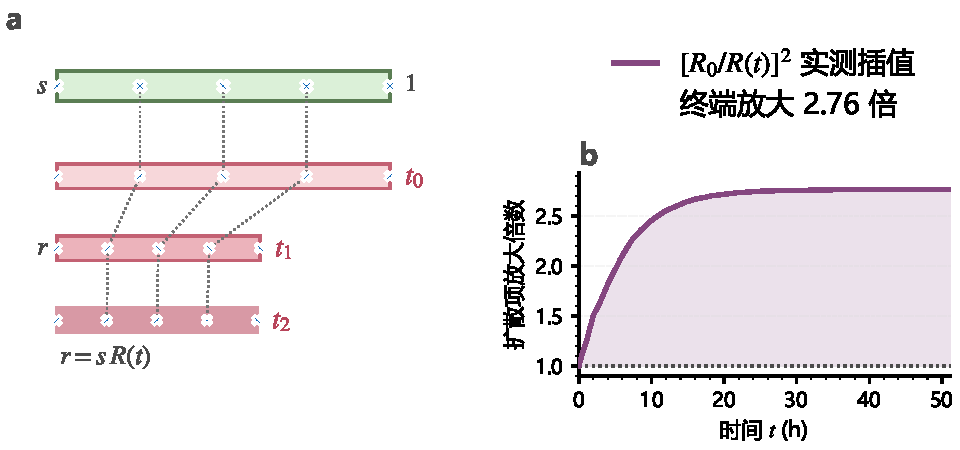
\includegraphics[width=0.9\textwidth,height=0.8\textheight,keepaspectratio]{../figures/fig_mech_moving.pdf}
  \caption{物质坐标映射与收缩放大。a：固定域上的节点随物质一起向轴线移动，
  表面恒落在 $s=1$；点线为同一物质点在三个时刻的轨迹。b：扩散项前
  $1/R^2(t)$ 的放大倍数随时间的变化，由附件 2 实测半径算出。}
  \label{fig:mech-moving}
\end{figure}

左图中三条点线是同一物质点在三个时刻的位置，它们都在向轴线靠拢，而其 $s$ 坐标不变，这正是“网格随物质移动”的含义；表面始终落在 $s=1$，边界条件的施加位置因此不随时间改变。右图给出收缩加速干燥的主要定量来源：半径由 $2$~cm 减到 $1.2$~cm 时，$1/R^2$ 增大 $2.78$ 倍，同样的含水率落差被压缩在更短的物理距离上，梯度随之增大；式~\eqref{eq:q4bc} 的 $1/R(t)$ 与控制体体积的变化同向叠加，量级小于此项。

物质坐标与实验室坐标是同一个方程的两种写法，数学上等价，本文选择前者是因为它把边界固定在坐标端点、且不需要用到半径的导数。作为独立对照，本文也按实验室坐标的写法实现了一支算例，用于交叉检验实现的正确性，两条路线的关系见图~\ref{fig:flow-q4}。

\begin{figure}[htbp]
  \centering
  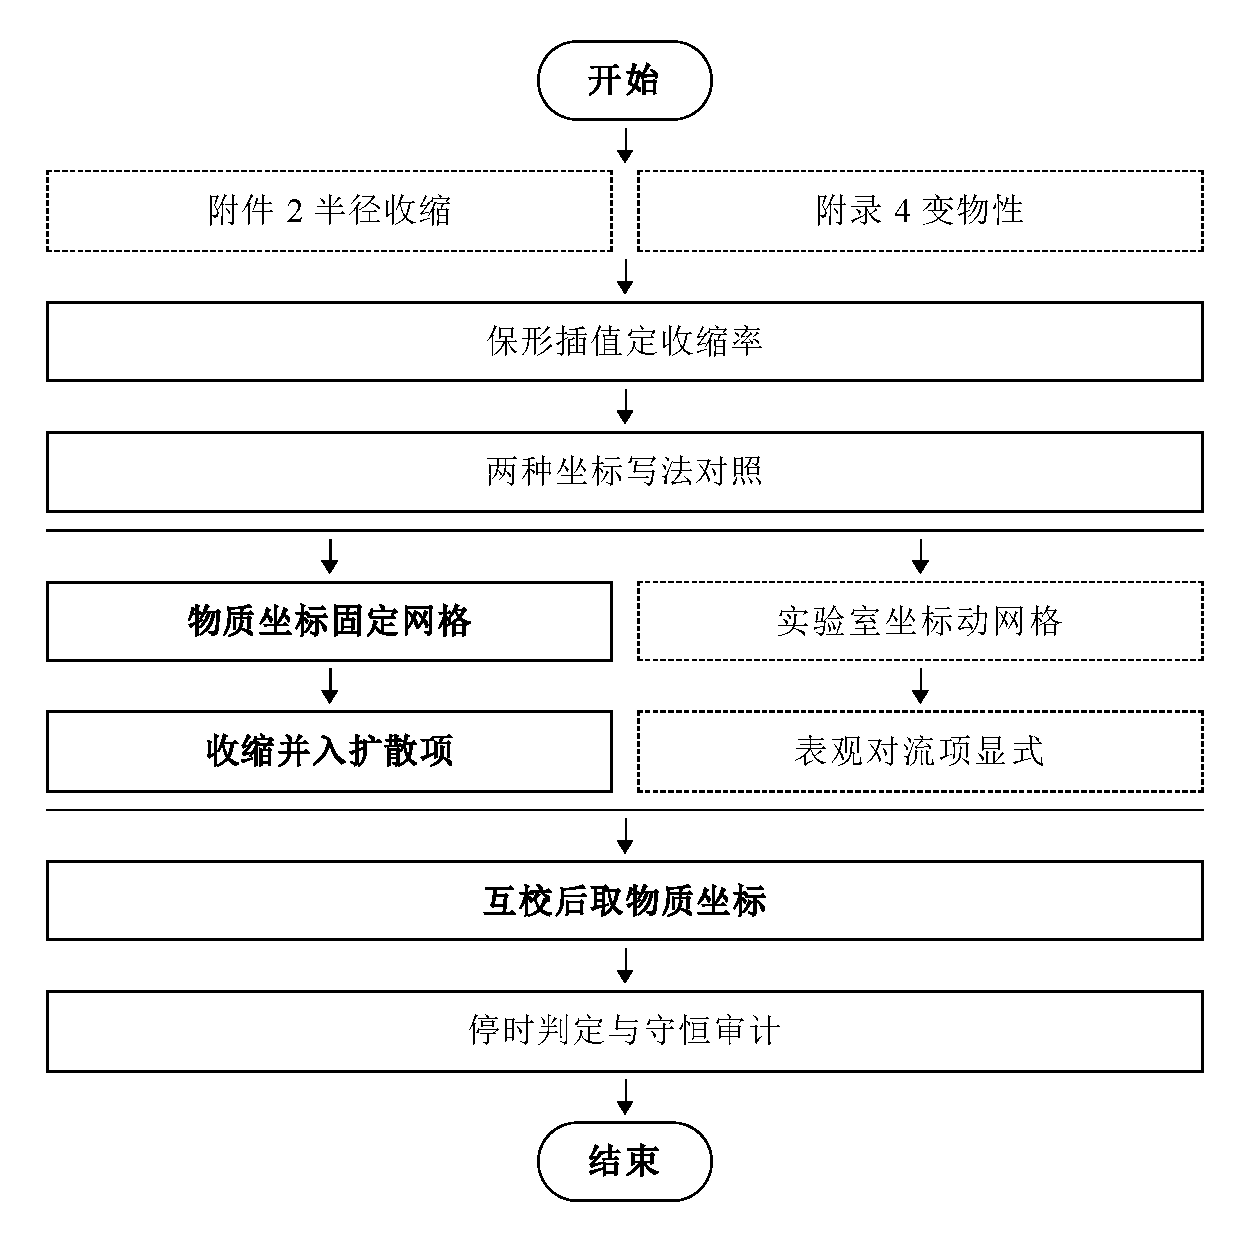
\includegraphics[width=0.8\textwidth,height=0.8\textheight,keepaspectratio]{../figures/fig_flow_q4.pdf}
  \caption{问题 4 收缩域的两条坐标路线。共同输入后分为物质坐标固定网格与实
  验室坐标动网格两支，收缩效应分别并入扩散项与显式表观对流项；加粗框为采纳的
  物质坐标支，虚线框为实验室坐标对照支，两支互校后取前者为主模型，再做停时判定
  与干物质守恒校核。}
  \label{fig:flow-q4}
\end{figure}

两支共用输入、物性、判据与求解器，仅在收缩效应的写法上分开。互校的判别标准取干物质守恒：单位长度的干物质总量在整个过程中不应改变。两支的残差与互校结果在第~\ref{sec:q34} 小节一并讨论。

\subsection{烘干时长与收缩域内的水分分布}

本问物性改用附录 4，即式~\eqref{eq:app4}，判据仍为式~\eqref{eq:tdry}、定位仍按式~\eqref{eq:interp}。所得烘干时长为

\begin{equation}
t_{\rm dry}=184098.165\ \mathrm{s}=51.1384\ \mathrm{h}=2.13\ \text{天},
\label{eq:tdry4}
\end{equation}

比问题三的 $57.5316$~h 提前 $6.3932$~h，相对减少 $11.11\%$，同样落在题目所述两到三天的区间内。该时刻半径为 $1.2000$~cm，收缩比恰为 $0.6000$；停时对应的时间 $1.84\times10^5$~s 落在附件 2 覆盖的 $72$~h 之内，无需对半径序列作任何外推。达标时刻表面含水率为 $0.0526$~kg/kg，截面平均含水率为 $0.118200$~kg/kg。

按题目要求给出的水分浓度结果列于表~\ref{tab:q4C}。

\begin{table}[H]
\centering
\caption{收缩情形下药材烘干过程的水分浓度（单位：kg/kg）}\label{tab:q4C}
\begin{tabular}{ccccccc}
\toprule
\multirow{2}{*}{时间/h} & \multicolumn{5}{c}{到药材中心的距离/cm} & \multirow{2}{*}{药材表面}\\
\cmidrule(lr){2-6}
 & 0 & 0.5 & 1 & 1.5 & 2 & \\
\midrule
6  & 1.7189 & 1.5366 & 1.0217 & --- & --- & 0.4205 \\
12 & 0.7383 & 0.6551 & 0.4086 & --- & --- & 0.1671 \\
18 & 0.4093 & 0.3690 & 0.2396 & --- & --- & 0.0893 \\
24 & 0.2854 & 0.2613 & 0.1788 & --- & --- & 0.0674 \\
30 & 0.2265 & 0.2095 & 0.1491 & --- & --- & 0.0595 \\
36 & 0.1930 & 0.1797 & 0.1315 & --- & --- & 0.0560 \\
42 & 0.1714 & 0.1604 & 0.1199 & --- & --- & 0.0541 \\
48 & 0.1562 & 0.1469 & 0.1115 & --- & --- & 0.0530 \\
烘干结束时间 & 0.1500 & 0.1412 & 0.1079 & --- & --- & 0.0526 \\
\bottomrule
\end{tabular}

\vspace{0.6em}
\begin{minipage}{0.96\textwidth}
\footnotesize 破折号表示该径向位置在对应时刻已落在药材之外：$6$~h 时半径已小于 $1.5$~cm，
故 $1.5$~cm 与 $2$~cm 两列此后不再有药材存在，按题意留空而不填零，以免与“已经很干”混淆。
末列“药材表面”跟随移动边界 $R(t)$ 取值。末行为式~\eqref{eq:tdry4} 给出的烘干结束时间
$t_{\rm dry}=51.1384$~h；与表~\ref{tab:q3C} 同理，该时刻判据量恰等于阈值 $0.1500$，
严格低于阈值在其后成立，下一个输出时刻（晚 $41.8$~s）轴线含水率为 $0.149979$~kg/kg。
\end{minipage}
\end{table}

与表~\ref{tab:q3C} 逐行对照可以看到，收缩情形下前 $6$~h 的轴线含水率还高于固定域（$1.7189$ 对 $1.0176$），说明附录 4 的扩散系数确实更小、初期干燥更慢；此后两者的差距逐步缩小，轴线含水率之比由 $6$~h 的 $1.69$ 降到 $24$~h 的 $1.20$、$36$~h 的 $1.04$，在 $36$ 至 $42$~h 之间才转为收缩情形更低（$42$~h 为 $0.99$，$48$~h 为 $0.97$），最终使总时长更短。这种先慢后快的交叉说明净时长的符号不能凭定性推理断定。收缩域内水分场的完整图景见图~\ref{fig:q4-contour}。

\begin{figure}[htbp]
  \centering
  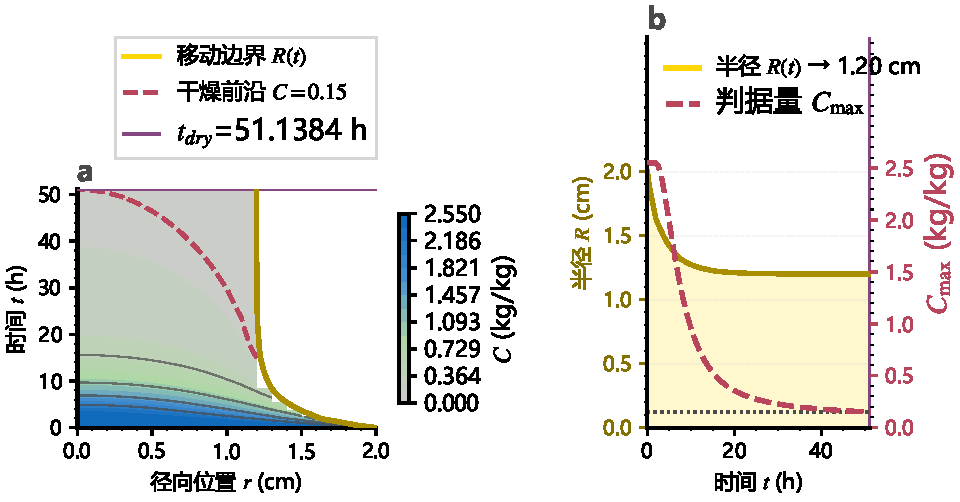
\includegraphics[width=0.9\textwidth,height=0.8\textheight,keepaspectratio]{../figures/fig_q4_contour.pdf}
  \caption{问题 4 收缩域内的水分场。a：$(r,t)$ 平面上的含水率等高线，实心区为
  药材本体，移动边界 $R(t)$ 右侧留白即已收缩掉的区域（不填零值以免与“很干”
  混淆）；粗虚线为干燥前沿 $C=0.15$，它与 $R(t)$ 的交汇决定停时。b：半径
  $R(t)$ 与判据量 $C_{\max}$ 的同步演化，竖线为停时；判据量在半径已趋平后
  才穿越阈值，说明停时由水分扩散而非几何收缩直接决定。}
  \label{fig:q4-contour}
\end{figure}

左图的留白区域是本图与图~\ref{fig:q3-frames} 最直观的差别：随着时间推移，药材本体在图上不断变窄，等值线被挤压向左，密集程度明显高于固定域的情形。右图的两条曲线揭示了一个容易误判的因果关系：半径在约 $35$~h 后已基本不再变化，而判据量还要再经过十余小时才穿越阈值，因此停时直接由水分扩散的进度决定，收缩的作用是在此之前就已经通过压缩扩散路径“预支”掉的。

\subsection{两个效应的分解与守恒校核}\label{sec:q34}

问题四与问题三的差别同时来自物性组的更换与几何的收缩。为把两者分开，本文在同一求解器、同一网格与同一判据下追加一个只换物性而保持半径不变的隔离算例，结果列于表~\ref{tab:q34}。

\begin{table}[H]
\centering
\caption{问题三到问题四的效应分解}\label{tab:q34}
\begin{tabular}{lcc}
\toprule
算例 & $t_{\rm dry}$/h & 相对上一行 \\
\midrule
问题三：附录 3 物性，固定半径 & 57.5316 & 基准 \\
只换附录 4 物性，半径仍固定 & 129.9252 & $+125.8\%$ \\
附录 4 物性并计入实测半径收缩 & 51.1384 & $-60.6\%$ \\
\bottomrule
\end{tabular}
\end{table}

两个效应的方向相反而量级都很大。附录 4 的扩散系数前因子比附录 3 小近一个数量级，虽然浓度项的指数更平缓（$-0.30/C$ 对 $-0.45/C$）能部分补偿，净效应仍使干燥慢一倍以上；几何收缩则通过 $1/R^2$ 把干燥加快约六成。表中两个百分数各以上一行为基准，因而是相继作用而非可以相加：$57.5316$~h 先被物性拉长到 $129.9252$~h，再被收缩压回 $51.1384$~h，最终相对问题三只提前 $11.1\%$。若只凭“收缩使干燥更快”就断言问题四明显快于问题三，或只凭“附录 4 扩散更弱”就断言更慢，都会得到错误结论。这一分解与守恒校核并列于图~\ref{fig:q34-compare}。

\begin{figure}[htbp]
  \centering
  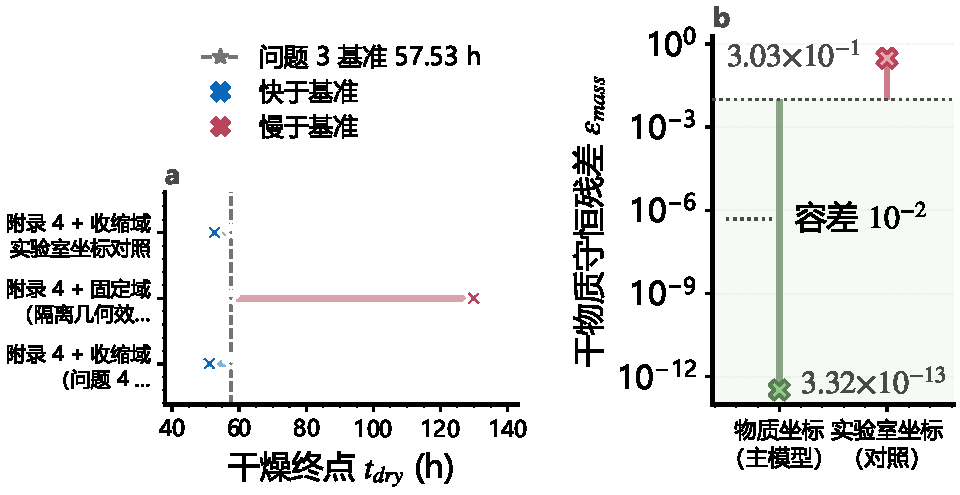
\includegraphics[width=0.9\textwidth,height=0.8\textheight,keepaspectratio]{../figures/fig_q34_compare.pdf}
  \caption{问题 3 与问题 4 的效应分解与实现校核。a：哑铃图，每行一个分支，
  左端固定为问题 3 的基准停时，右端为该分支实算值，连线长度即该处理的净效应；
  可见单换附录 4 物性（固定域）使干燥显著变慢，再叠加半径收缩才把停时拉回并
  超过基准，两个效应方向相反。b：两支实现的干物质守恒残差，以 $10^{-2}$
  容差线为基线的杆状图（对数纵轴上柱长会随人为地板而变，故不用柱状）；物质
  坐标残差处于舍入量级，实验室坐标一支达 30\%，据此定位到该支把已被坐标变换
  吸收的边界运动又显式计入了一次。}
  \label{fig:q34-compare}
\end{figure}

左图把表~\ref{tab:q34} 画成哑铃形式，两条连线一长一短、方向相反，长度差即最终的净效应。右图是干物质守恒的校核结果，它的作用超出了常规校验。物质坐标一支的残差为 $3.3\times10^{-13}$，处于浮点舍入累积的量级；实验室坐标一支却达到 $30.3\%$，远超 $1\%$ 的容差。既然两种写法在数学上等价，这样悬殊的差别只能来自实现本身。据此复查发现，该支在保留表观对流项的同时，扩散项仍按物质坐标的形式带有 $1/R^2$ 因子，等于把边界运动计入了两次，其停时因而系统性偏慢 $2.93\%$（$52.6377$~h）。这里记录这一诊断，是因为它说明守恒校核能捕捉到单纯比较停时数值无法发现的实现错误，而不是说明某一种坐标写法本身更优。

收缩方式本身也可以由守恒关系独立判定。单位长度的干物质总量守恒给出

\begin{equation}
\rho_{\rm d}(t)\,R^2(t)=\rho_{\rm d}(0)\,R^2(0),\qquad
\rho_{\rm d}=\frac{\rho(C)}{1+C},
\label{eq:drymass}
\end{equation}

由附录 4 的密度公式与初始含水率得 $\rho_{\rm d}(0)=278.73$~kg/m$^3$。把停时处的收缩比 $R(t_{\rm dry})/R_0=0.6000$ 代入式~\eqref{eq:drymass}，若按径向仿射收缩反推，干物质密度为 $774.26$~kg/m$^3$；若改按各向同性收缩反推，则为 $1290.43$~kg/m$^3$。这两个数值需要与附录 4 密度公式的两个自然参照相比：其一是含水率趋零时的绝干截距 $760$~kg/m$^3$，径向收缩偏高 $1.9\%$，各向同性收缩偏高 $69.8\%$；其二是按终态平均含水率算得的 $\rho(\bar C)/(1+\bar C)=689.18$~kg/m$^3$，径向收缩偏高 $12.35\%$，各向同性收缩偏高 $87.24\%$。两个参照下的结论一致：径向仿射收缩与题给数据相容到十几个百分点以内，各向同性收缩则偏离近一倍，据此排除后者。这一判断使用的是附件 2 的几何序列与附录 4 的密度公式两项互不相干的题给信息，因而构成对假设（6）的独立支持。
